\documentclass[10pt,twocolumn,letterpaper]{article}

\usepackage{cvpr}
\usepackage{times}
\usepackage{epsfig}
\usepackage{graphicx}
\usepackage{amsmath}
\usepackage{amssymb}
\usepackage{url}
\usepackage{listings}
\usepackage{xcolor}
\usepackage{float}

% Code listing style
\lstset{
  basicstyle=\ttfamily\scriptsize,
  breaklines=true,
  frame=single,
  language=C++,
  keywordstyle=\color{blue},
  commentstyle=\color{green!60!black},
  stringstyle=\color{red},
  numbers=none,
  showstringspaces=false,
  tabsize=2,
  breakatwhitespace=true,
  postbreak=\mbox{\textcolor{gray}{$\hookrightarrow$}\space}
}

\cvprfinalcopy

\def\cvprPaperID{****}
\def\httilde{\mbox{\tt\raisebox{-.5ex}{\symbol{126}}}}

\ifcvprfinal\pagestyle{empty}\fi
\begin{document}

%%%%%%%%% TITLE
\title{N-gram Histogram Computation\\Parallel Computing 2025-2026 --- Mid-Term Assignment}

\author{Mattia Manneschi\\
{\tt\small mattia.manneschi@edu.unifi.it}
}

\maketitle
\thispagestyle{empty}

%%%%%%%%% ABSTRACT
\begin{abstract}
This assignment demonstrates how to implement parallel n-gram (bigrams/trigrams) counting on text corpora using OpenMP. The project implements multiple parallelization strategies and compares their performance against a sequential baseline. The analysis includes thread scaling, workload scaling, and frequency distribution statistics following Zipf's Law for both bigrams and trigrams.
\end{abstract}

%%%%%%%%% BODY TEXT
\noindent\large\textbf{Future Distribution Permission}\\
\indent The author(s) of this report give permission for this document to be distributed to Unifi-affiliated students taking future courses.

\section{Introduction}

This project implements a parallel n-gram counting system for text analysis, leveraging multi-core CPU parallelism through OpenMP. The main objective is to demonstrate the benefits of different parallelization strategies for computationally intensive text processing operations.

N-gram analysis is a fundamental technique in Natural Language Processing (NLP), used for language modeling, text classification, spell checking, and information retrieval. An n-gram is a contiguous sequence of n items (characters or words) from a text. Computing frequency histograms of n-grams requires processing large amounts of text data, making it an ideal candidate for parallelization.

The dataset used during experiments consists of public domain texts from Project Gutenberg, providing a realistic corpus for performance evaluation.

\subsection{Project Objectives}

\begin{itemize}
\item Implement a sequential CPU version as baseline for performance comparison.
\item Develop multiple OpenMP parallelization strategies with different optimization approaches.
\item Conduct complete performance analysis with thread scaling and workload scaling tests.
\item Generate frequency distributions and verify Zipf's Law on natural language text.
\item Compare results between bigrams ($n=2$) and trigrams ($n=3$).
\end{itemize}

\section{Theoretical Background}

\subsection{N-gram Definition}

An n-gram is a contiguous sequence of $n$ items from a given text. For word-level n-grams, a bigram ($n=2$) consists of two consecutive words, while a trigram ($n=3$) consists of three consecutive words. Given a text with $W$ words, the number of possible n-grams is $W - n + 1$.

For example, given the sentence ``the quick brown fox'', the word bigrams are: ``the quick'', ``quick brown'', ``brown fox'', while the trigrams are: ``the quick brown'', ``quick brown fox''.

\subsection{Zipf's Law}

Zipf's Law states that in natural language text, the frequency of a word is inversely proportional to its rank in the frequency table. Mathematically:
\begin{equation}
f(r) \propto \frac{1}{r}
\end{equation}
where $f$ is frequency and $r$ is rank. This means a few n-grams appear very frequently, while most n-grams appear only once or twice.

Key metrics for Zipf analysis include: Hapax legomena (n-grams appearing exactly once), Dis legomena (n-grams appearing exactly twice), and Coverage (percentage of total tokens covered by the top-K most frequent n-grams).

\subsection{OpenMP Parallelization}

OpenMP (Open Multi-Processing) is an API for shared-memory parallel programming. Key concepts used in this project include: Thread-Level Storage (TLS) where each thread maintains private data structures, parallel for loops with automatic distribution of iterations, reduction operations for combining partial results, and scheduling strategies (static, dynamic, guided).

\section{Implementation}

\subsection{Project Structure}

The project is organized in modules: \texttt{main\_driver.cpp} (benchmark orchestration), \texttt{ngram\_counter.cpp} (sequential and parallel implementations), \texttt{data\_loader.cpp} (text loading and tokenization), \texttt{statistics.cpp} (frequency distribution analysis), and \texttt{results\_exports.cpp} (CSV output generation). The experiments were conducted using an AMD Ryzen 7 2700X CPU with 8 cores and 16 threads.

\subsection{Sequential Implementation (Baseline)}

The sequential implementation processes the entire corpus in a single thread. For each position in the word array, it constructs the n-gram string and updates a hash map counter. This version serves as the baseline for speedup calculations.

\begin{lstlisting}
Histogram count_seq(
    const std::vector<std::string>& words,
    const int n_gram_size)
{
  Histogram hist;
  if (words.size() < 
      static_cast<size_t>(n_gram_size)) 
    return hist;
  for (size_t i = 0; 
       i <= words.size() - n_gram_size; ++i)
  {
    std::string n_gram = words[i];
    for (int j = 1; j < n_gram_size; ++j)
    {
      n_gram += " " + words[i + j];
    }
    hist[n_gram]++;
  }
  return hist;
}
\end{lstlisting}

\subsection{Parallel Implementations}

Six parallel strategies were implemented, divided into two categories based on their optimization target.

\subsubsection{Thread Scaling Strategies}

The following three implementations are optimized for thread scaling tests, where the workload is fixed and the number of threads varies. They focus on minimizing synchronization overhead and balancing I/O with computation.

\textbf{Single Reader - Worker TLS:} A single thread reads all documents using \texttt{\#pragma omp single} while other threads wait, then all threads process the loaded texts in parallel with thread-local histograms.

\begin{lstlisting}
void count_par_singleReader_Worker_TLS(
    int n_gram_size, int max_iter)
{
  std::vector<std::string> texts;
  Histogram hist;
  #pragma omp parallel shared(texts, 
      max_iter, n_gram_size, hist) 
      default(none)
  {
    Histogram thread_word_hist;
    for (int k = 0; k < max_iter; k++)
    {
      for (const auto& document : 
          std::filesystem::directory_iterator(
            "data/Texts"))
      {
        std::string document_path = 
            document.path().string();
        std::ifstream file(document_path);
        #pragma omp single
        {
          if (file.is_open())
          {
            std::stringstream buffer;
            buffer << file.rdbuf();
            texts.push_back(buffer.str());
            file.close();
          }
        }
      }
    }
    #pragma omp for nowait schedule(dynamic,1)
    for (auto& text : texts)
      UpdateHistogramWord(thread_word_hist, 
          text, n_gram_size);
    #pragma omp critical (word)
    for (const auto& [fst, snd] : 
        thread_word_hist)
      hist[fst] += snd;
  }
}
\end{lstlisting}

\textbf{On the Fly - Parallel I/O:} Each thread reads and processes documents independently as they are assigned. File paths are constructed using document index, and each thread maintains its own histogram.

\begin{lstlisting}
void count_par_onTheFly_parallelIO(
    const int n_gram_size, int max_iter)
{
  int doc_count = 0;
  for (const auto& document : 
      std::filesystem::directory_iterator(
        "data/Texts"))
    doc_count++;
  Histogram hist;
  #pragma omp parallel shared(doc_count, 
      max_iter, n_gram_size, hist) 
      default(none)
  {
    Histogram thread_word_histogram;
    for (int k = 0; k < max_iter; k++)
    {
      #pragma omp for nowait schedule(dynamic,1)
      for (int i = 0; i < doc_count; i++)
      {
        std::string document_path = 
            "data/Texts/" + std::to_string(i) 
            + ".txt";
        if (std::ifstream file(document_path); 
            file.is_open())
        {
          std::stringstream buffer;
          buffer << file.rdbuf();
          UpdateHistogramWord(
              thread_word_histogram, 
              buffer.str(), n_gram_size);
          file.close();
        }
      }
    }
    #pragma omp critical (word)
    for (const auto& [fst, snd] : 
        thread_word_histogram)
      hist[fst] += snd;
  }
}
\end{lstlisting}

\textbf{Hybrid Preload TLS:} Each thread loads documents into its own local vector, then processes them sequentially. This combines parallel I/O with complete thread isolation for both data and histograms.

\begin{lstlisting}
void count_par_hybrid_preload_TLS(
    int n_gram_size, int max_iter)
{
  int doc_count = 0;
  for (const auto& document : 
      std::filesystem::directory_iterator(
        "data/Texts"))
    doc_count++;
  Histogram hist;
  #pragma omp parallel shared(doc_count, 
      max_iter, n_gram_size, hist) 
      default(none)
  {
    std::vector<std::string> texts;
    Histogram thread_word_histogram;
    for (int k = 0; k < max_iter; k++)
    {
      #pragma omp for nowait schedule(dynamic,1)
      for (int i = 0; i < doc_count; i++)
      {
        std::string document_path = 
            "data/Texts/" + std::to_string(i) 
            + ".txt";
        if (std::ifstream file(document_path); 
            file.is_open())
        {
          std::stringstream buffer;
          buffer << file.rdbuf();
          texts.push_back(buffer.str());
          file.close();
        }
      }
    }
    for (size_t l = 0; l < texts.size(); l++)
      UpdateHistogramWord(
          thread_word_histogram, 
          texts[l], n_gram_size);
    #pragma omp critical (word)
    for (const auto& [fst, snd] : 
        thread_word_histogram)
      hist[fst] += snd;
  }
}
\end{lstlisting}

\subsubsection{Workload Scaling Strategies}

The following three implementations are optimized for workload scaling tests, where the number of threads is fixed and the workload size varies (via multiplier). They focus on efficiently handling large datasets and minimizing memory contention.

\textbf{Document Level TLS:} Documents are tokenized in parallel first, then each thread processes a subset of tasks (document $\times$ multiplier combinations) using dynamic scheduling. Uses optimized helper functions and pre-allocated histogram capacity.

\begin{lstlisting}
Histogram count_par_document_level_tls(
    const std::string& directory_path,
    int ngram_size, int num_threads, 
    int multiplier)
{
  // Collect file paths
  std::vector<fs::path> file_paths;
  for (const auto& entry : 
      fs::directory_iterator(directory_path))
    if (entry.is_regular_file() && 
        entry.path().extension() == ".txt")
      file_paths.push_back(entry.path());
  const size_t num_docs = file_paths.size();
  const size_t total_tasks = num_docs * 
      static_cast<size_t>(multiplier);
  // Phase 1: Parallel tokenization
  std::vector<std::vector<std::string>> 
      tokenized_docs(num_docs);
  #pragma omp parallel for \
      num_threads(num_threads) schedule(dynamic)
  for (size_t i = 0; i < num_docs; ++i)
    tokenized_docs[i] = tokenize_text(
        read_file_fast(file_paths[i]));
  // Phase 2: Parallel counting with TLS
  std::vector<Histogram> 
      local_hists(num_threads);
  #pragma omp parallel num_threads(num_threads)
  {
    const int tid = omp_get_thread_num();
    Histogram& my_hist = local_hists[tid];
    std::string ngram_buffer;
    ngram_buffer.reserve(128);
    #pragma omp for schedule(dynamic, 4)
    for (size_t task_id = 0; 
        task_id < total_tasks; ++task_id)
    {
      const size_t doc_idx = task_id % num_docs;
      const std::vector<std::string>& words = 
          tokenized_docs[doc_idx];
      for (size_t k = 0; 
          k <= words.size() - ngram_size; ++k)
      {
        build_ngram_inplace(words, k, 
            ngram_size, ngram_buffer);
        my_hist[ngram_buffer]++;
      }
    }
  }
  // Merge local histograms and return
  // ...
}
\end{lstlisting}

\textbf{Fine-Grained Locking:} Uses a sharded hash table with 1024 independent shards, each protected by its own OpenMP lock. N-grams are hashed to determine the shard, reducing lock contention compared to a single global lock.

\begin{lstlisting}
void count_par_fine_grained_locking(
    const std::string& directory_path,
    int n_gram_size, int num_threads, 
    int multiplier)
{
  // Load and tokenize documents, 
  // build all_words vector
  // ...
  constexpr int NUM_SHARDS = 1024;
  std::vector<Histogram> shards(NUM_SHARDS);
  std::vector<omp_lock_t> 
      shard_locks(NUM_SHARDS);
  for (auto& l : shard_locks)
    omp_init_lock(&l);
  const size_t limit = 
      all_words.size() - n_gram_size;
  #pragma omp parallel num_threads(num_threads)\
      default(none) shared(all_words, \
      n_gram_size, shards, shard_locks, limit)
  {
    #pragma omp for schedule(static)
    for (size_t i = 0; i <= limit; ++i)
    {
      std::string n_gram = all_words[i];
      for (int j = 1; j < n_gram_size; ++j)
        n_gram += " " + all_words[i + j];
      const size_t h = 
          std::hash<std::string>{}(n_gram);
      const size_t shard_id = h % NUM_SHARDS;
      omp_set_lock(&shard_locks[shard_id]);
      shards[shard_id][n_gram]++;
      omp_unset_lock(&shard_locks[shard_id]);
    }
  }
  for (auto& l : shard_locks)
    omp_destroy_lock(&l);
}
\end{lstlisting}

\textbf{Chunk-Based Adaptive:} The corpus is divided into chunks with size automatically calculated based on thread count (target: 6 chunks per thread). Uses dynamic scheduling for load balancing, with each thread maintaining a local histogram.

\begin{lstlisting}
void count_par_chunk_based_adaptive(
    const std::string& directory_path,
    int ngram_size, int num_threads, 
    int multiplier)
{
  // Load files and build corpus vector
  // ...
  const size_t num_ngrams = 
      corpus_size - ngram_size + 1;
  const size_t target_chunks_per_thread = 6;
  const size_t target_total_chunks = 
      num_threads * target_chunks_per_thread;
  size_t chunk_size = std::max(
      static_cast<size_t>(1000),
      num_ngrams / target_total_chunks);
  const size_t num_chunks = 
      (num_ngrams + chunk_size - 1) / chunk_size;
  std::vector<Histogram> 
      local_hists(num_threads);
  #pragma omp parallel num_threads(num_threads)
  {
    const int tid = omp_get_thread_num();
    Histogram& my_hist = local_hists[tid];
    std::string ngram_buffer;
    ngram_buffer.reserve(128);
    #pragma omp for schedule(dynamic)
    for (size_t chunk_id = 0; 
        chunk_id < num_chunks; ++chunk_id)
    {
      const size_t start_ngram = 
          chunk_id * chunk_size;
      const size_t end_ngram = std::min(
          start_ngram + chunk_size, num_ngrams);
      for (size_t k = start_ngram; 
          k < end_ngram; ++k)
      {
        build_ngram_inplace(corpus, k, 
            ngram_size, ngram_buffer);
        my_hist[ngram_buffer]++;
      }
    }
  }
  // Merge local histograms
}
\end{lstlisting}

\subsection{Helper Functions}

Several helper functions are used across the implementations for text processing and n-gram construction.

\textbf{tokenize\_text:} Converts raw text to a vector of lowercase words, using SIMD vectorization for character processing:

\begin{lstlisting}
std::vector<std::string> tokenize_text(
    const std::string& text)
{
  std::vector<std::string> words;
  std::string processed_text = text;
  #pragma omp simd
  for (size_t i = 0; 
      i < processed_text.length(); ++i)
    processed_text[i] = 
        std::tolower(processed_text[i]);
  #pragma omp simd
  for (size_t i = 0; 
      i < processed_text.length(); ++i)
  {
    char c = processed_text[i];
    if (std::ispunct(c) || c == '\n' 
        || c == '\t')
      processed_text[i] = ' ';
  }
  std::stringstream ss(processed_text);
  std::string word;
  while (ss >> word)
    if (!word.empty())
      words.push_back(word);
  return words;
}
\end{lstlisting}

\textbf{UpdateHistogramWord:} Used by thread scaling strategies to tokenize text and update histogram in one step:

\begin{lstlisting}
void UpdateHistogramWord(Histogram& hist, 
    const std::string& text, 
    const int n_gram_size)
{
  std::istringstream stream(text);
  const std::vector<std::string> words(
      (std::istream_iterator<std::string>(
        stream)), {});
  if (words.size() > 
      static_cast<size_t>(n_gram_size))
  {
    for (size_t i = 0; 
        i <= words.size() - n_gram_size; ++i)
    {
      std::string word_string;
      for (size_t j = i; 
          j < i + n_gram_size - 1; ++j)
        word_string += words[j] + " ";
      word_string += words[i + n_gram_size - 1];
      for (char& ch : word_string) 
        ch = std::tolower(ch);
      word_string.erase(
          std::remove_if(word_string.begin(), 
            word_string.end(),
            [](char ch) { 
              return !std::isalpha(ch) 
                  && ch != ' '; }),
          word_string.end());
      hist[word_string]++;
    }
  }
}
\end{lstlisting}

\textbf{read\_file\_fast and build\_ngram\_inplace:} Optimized functions used by workload scaling strategies:

\begin{lstlisting}
static std::string read_file_fast(
    const fs::path& filepath)
{
  std::ifstream file(filepath, 
      std::ios::binary | std::ios::ate);
  if (!file.is_open()) return "";
  auto size = file.tellg();
  file.seekg(0, std::ios::beg);
  std::string content(
      static_cast<size_t>(size), '\0');
  file.read(&content[0], size);
  return content;
}

static void build_ngram_inplace(
    const std::vector<std::string>& words,
    size_t start_idx, int ngram_size, 
    std::string& buffer)
{
  buffer.clear();
  buffer.append(words[start_idx]);
  for (int j = 1; j < ngram_size; ++j)
  {
    buffer.push_back(' ');
    buffer.append(words[start_idx + j]);
  }
}
\end{lstlisting}

\section{Experimental Results}

\subsection{Test Methodology}

Benchmarks were executed using texts from Project Gutenberg, totaling over 18 million n-gram tokens. Two types of scaling tests were conducted: Thread Scaling (fixed workload, varying threads from 1 to 16) and Workload Scaling (fixed 16 threads, varying workload multiplier from 1x to 10x). Tests were performed for both bigrams ($n=2$) and trigrams ($n=3$).

\subsection{Bigram (2-gram) Results}

\textbf{Thread Scaling:} Figure~\ref{fig:bigram_thread} shows the speedup achieved by three parallelization strategies as the number of threads increases.

\begin{figure}[H]
\centering
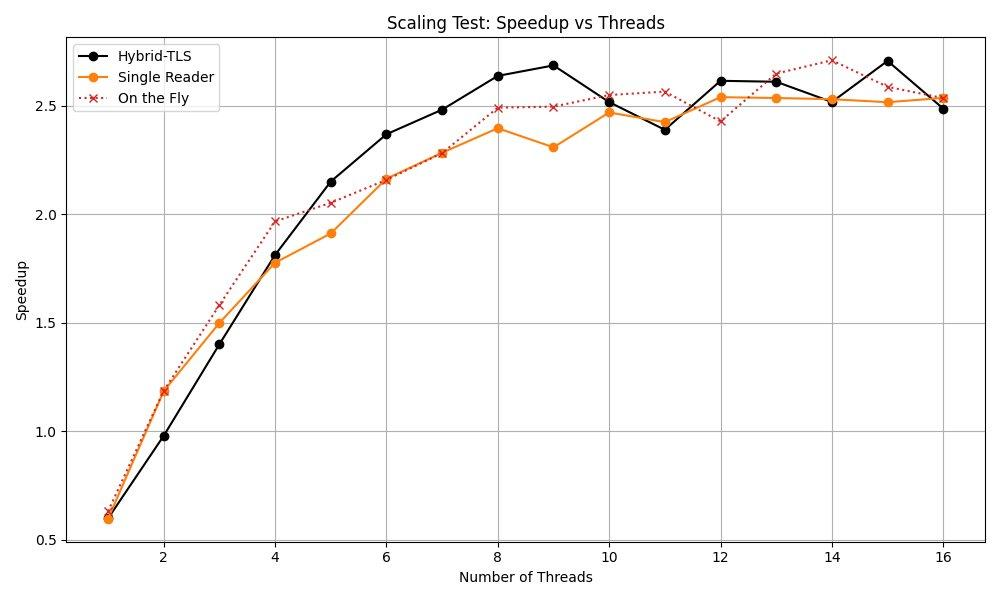
\includegraphics[width=0.9\linewidth]{figures/image2.jpg}
\caption{Bigram Thread Scaling: Speedup vs Number of Threads}
\label{fig:bigram_thread}
\end{figure}

All three strategies show similar scaling behavior, reaching maximum speedup around 2.5-2.7x with 8-10 threads. The Hybrid-TLS strategy achieves slightly better peak performance (2.7x at 9 threads). Beyond 10 threads, speedup plateaus due to memory bandwidth saturation.

\textbf{Workload Scaling:} Figure~\ref{fig:bigram_workload} shows how speedup improves with increasing workload size.

\begin{figure}[H]
\centering
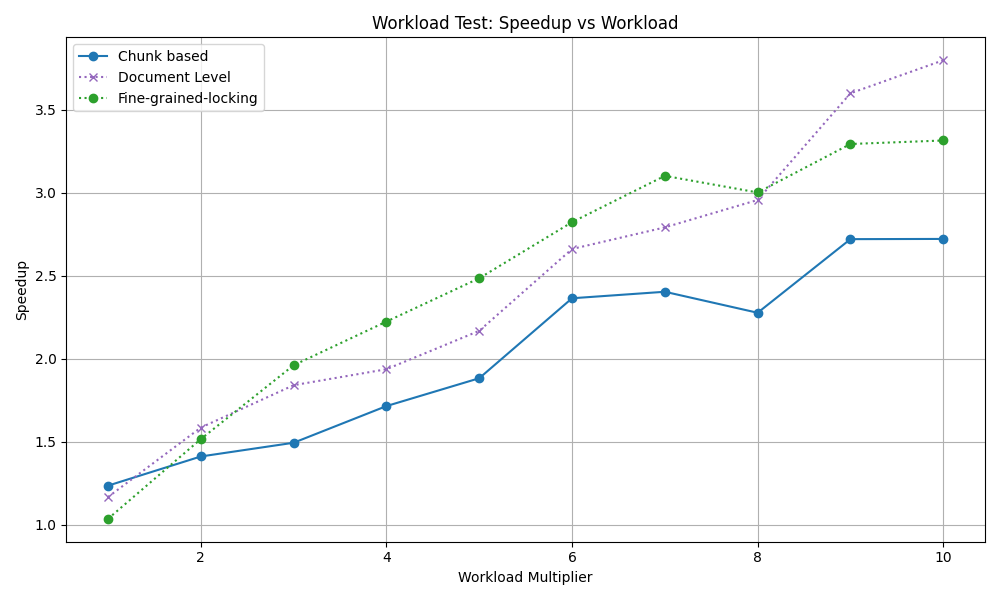
\includegraphics[width=0.9\linewidth]{figures/image10.png}
\caption{Bigram Workload Scaling: Speedup vs Workload Multiplier}
\label{fig:bigram_workload}
\end{figure}

Document Level achieves the best speedup at high workloads (3.9x at 10x multiplier), followed by Fine-grained-locking (3.3x) and Chunk-based (2.7x). Larger problem sizes better amortize parallelization overhead.

\textbf{Frequency Distribution:} Figure~\ref{fig:bigram_zipf} shows the Zipf's Law analysis for bigrams.

\begin{figure}[H]
\centering
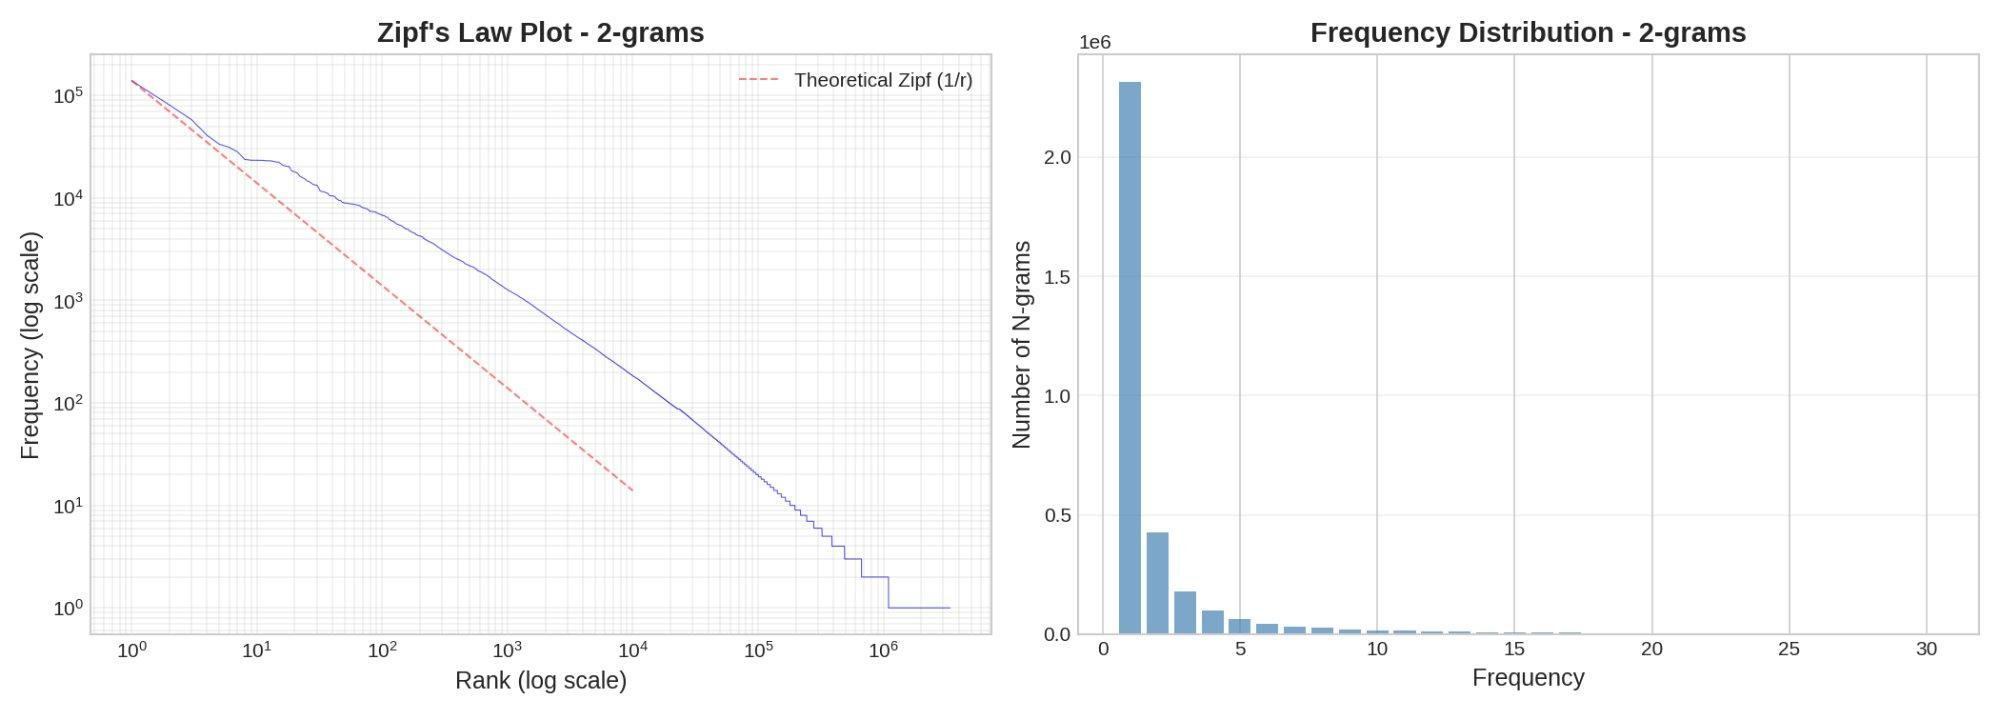
\includegraphics[width=0.9\linewidth]{figures/image4.jpg}
\caption{Bigram Zipf's Law Plot and Frequency Distribution}
\label{fig:bigram_zipf}
\end{figure}

The data closely follows the theoretical Zipf distribution. The histogram shows extreme skewness: over 2.3 million bigrams appear only once.

\textbf{Top Bigrams:} Figure~\ref{fig:bigram_top} shows the 20 most frequent bigrams.

\begin{figure}[H]
\centering
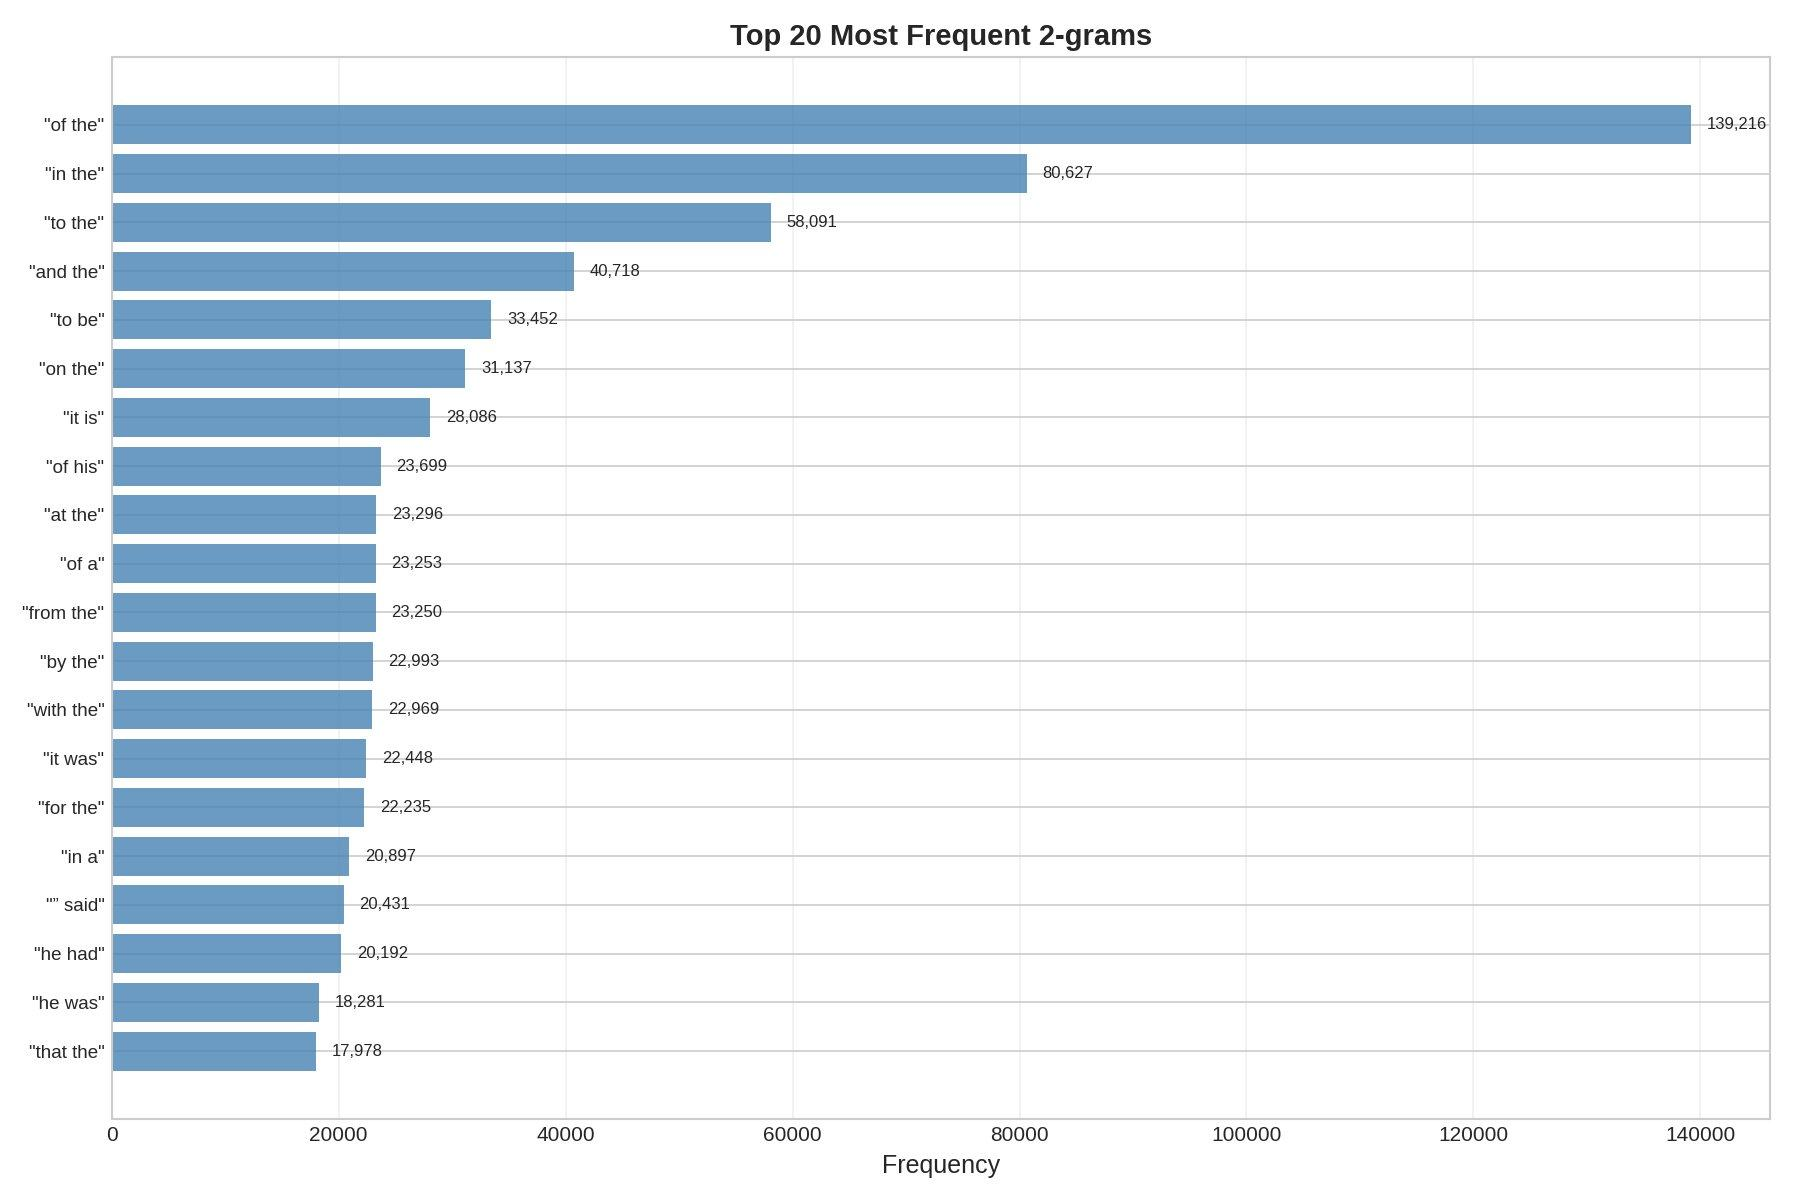
\includegraphics[width=0.9\linewidth]{figures/image9.jpg}
\caption{Top 20 Most Frequent Bigrams}
\label{fig:bigram_top}
\end{figure}

The most frequent bigram is ``of the'' with 139,216 occurrences, followed by ``in the'' (80,627) and ``to the'' (58,091). These function word combinations dominate English text.

\textbf{Statistics Summary:} Figure~\ref{fig:bigram_stats} presents the complete bigram analysis summary.

\begin{figure}[H]
\centering
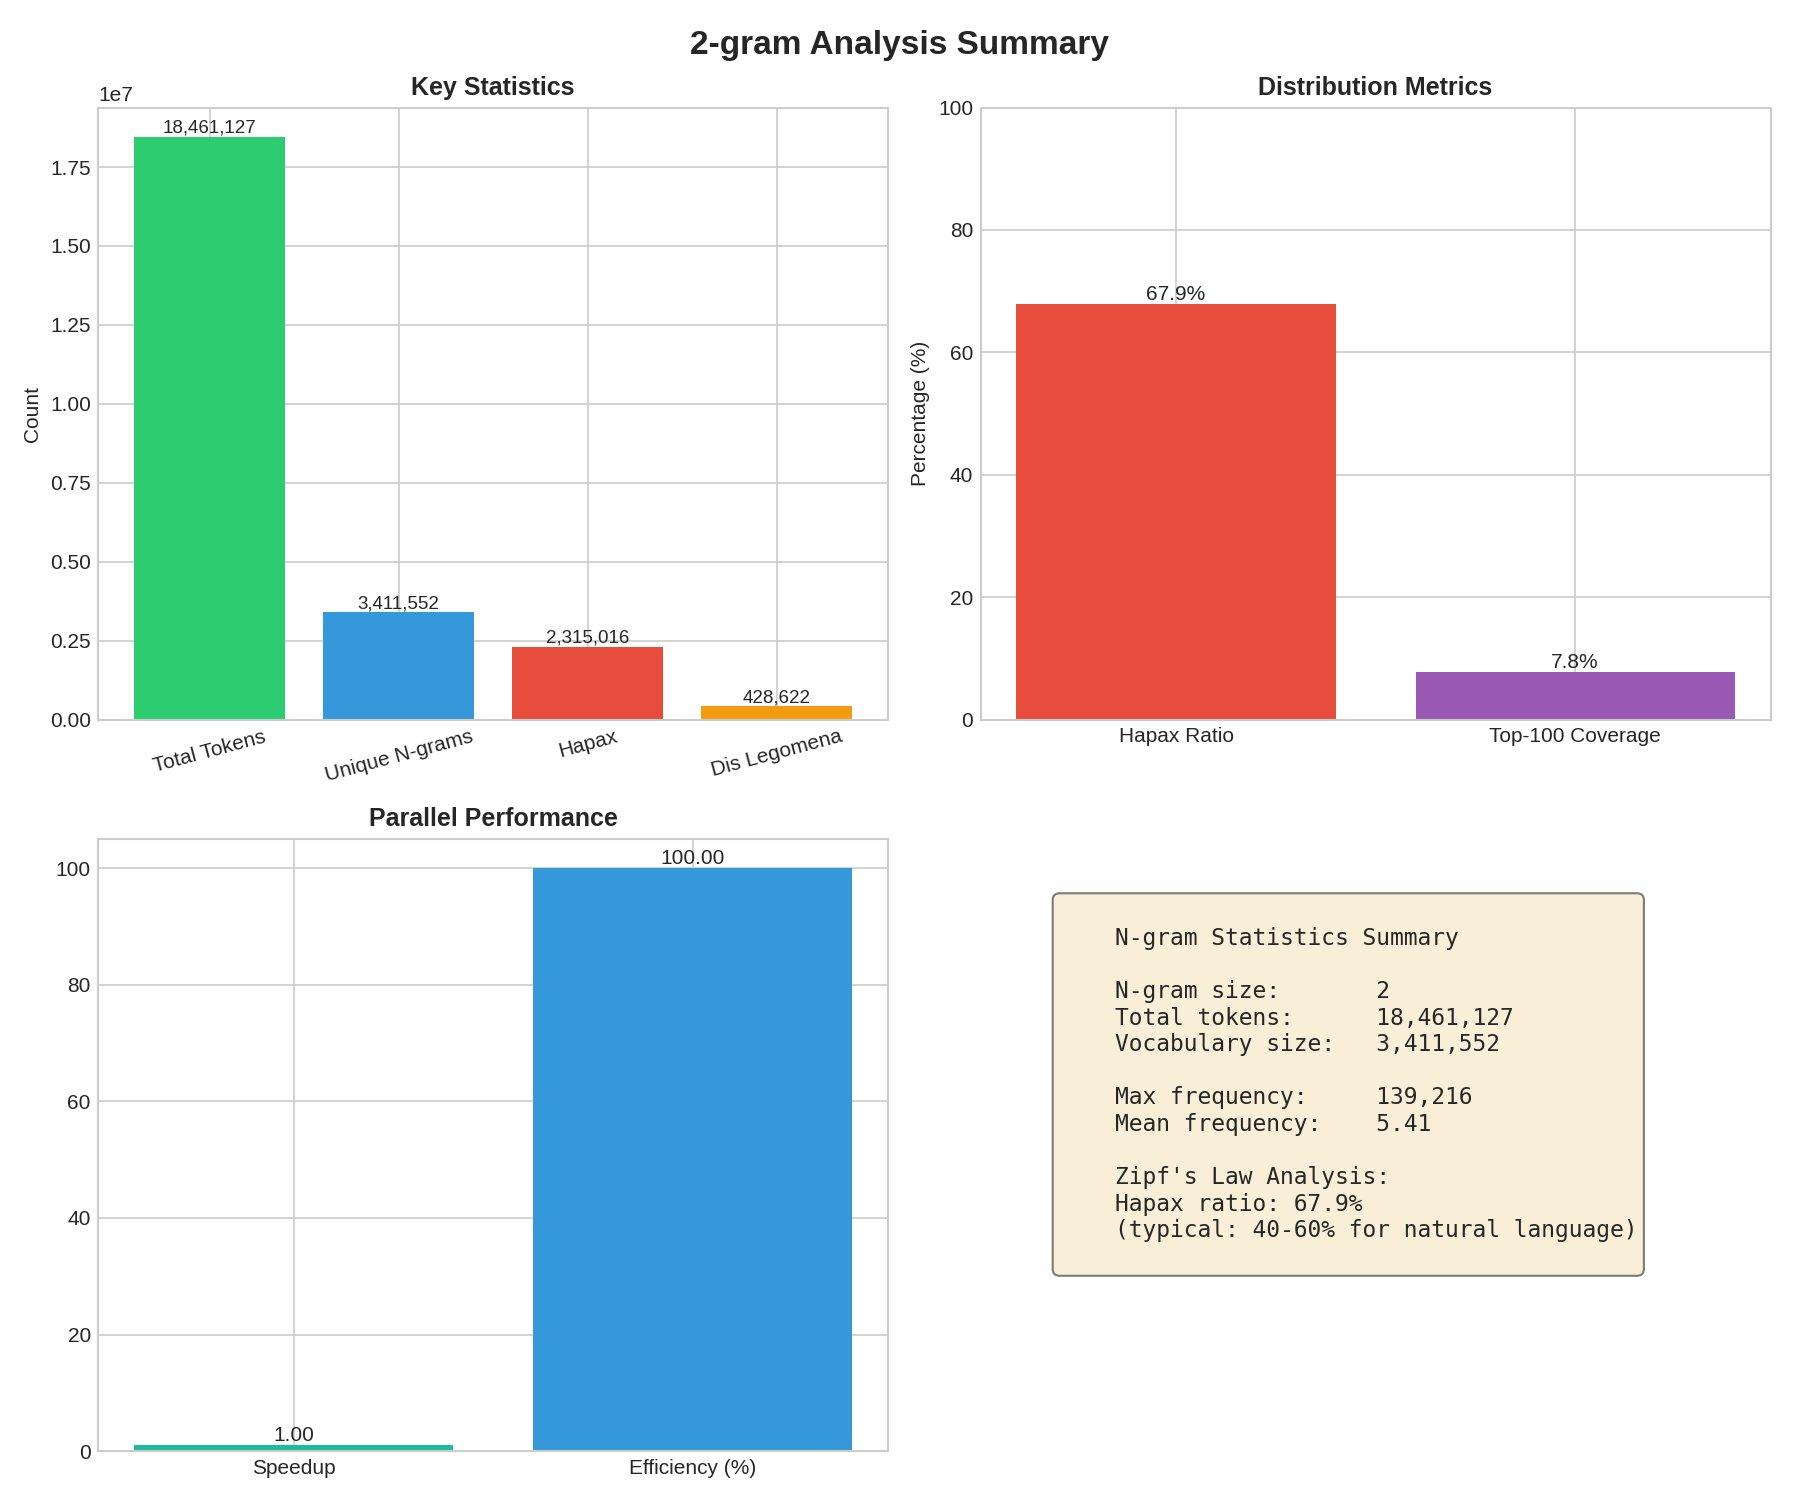
\includegraphics[width=0.9\linewidth]{figures/image6.jpg}
\caption{Bigram Analysis Summary}
\label{fig:bigram_stats}
\end{figure}

Key statistics: 18,461,127 total tokens, 3,411,552 unique bigrams, 67.9\% hapax ratio, mean frequency 5.41.

\subsection{Trigram (3-gram) Results}

\textbf{Thread Scaling:} Figure~\ref{fig:trigram_thread} shows thread scaling for trigram counting, which presents different characteristics than bigrams.

\begin{figure}[H]
\centering
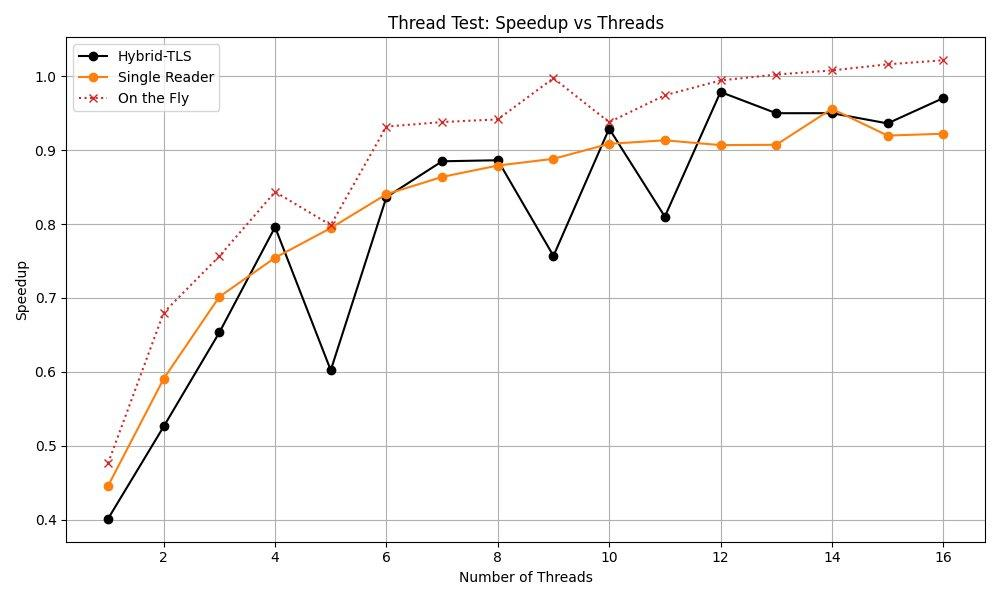
\includegraphics[width=0.9\linewidth]{figures/image5.jpg}
\caption{Trigram Thread Scaling: Speedup vs Number of Threads}
\label{fig:trigram_thread}
\end{figure}

Trigram counting shows speedup values below 1.0 for lower thread counts, indicating the parallel overhead exceeds the benefits. Performance improves gradually, reaching approximately 1.0x speedup at 16 threads. This is due to the much larger vocabulary (10M+ unique trigrams) causing significant hash table overhead and cache misses.

\textbf{Workload Scaling:} Figure~\ref{fig:trigram_workload} shows workload scaling for trigrams.

\begin{figure}[H]
\centering
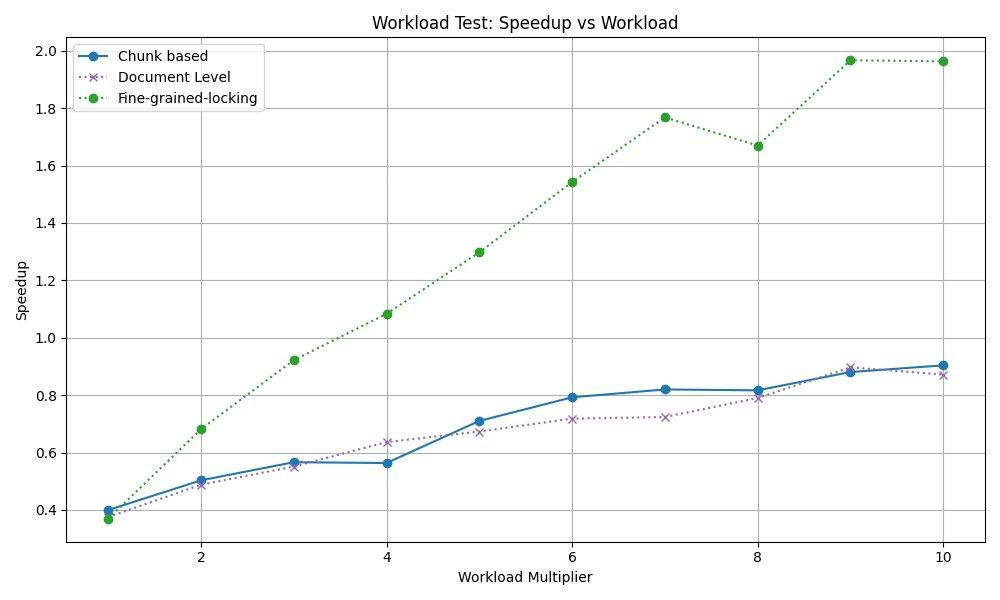
\includegraphics[width=0.9\linewidth]{figures/image1.jpg}
\caption{Trigram Workload Scaling: Speedup vs Workload Multiplier}
\label{fig:trigram_workload}
\end{figure}

Fine-grained-locking performs best for trigrams, reaching 1.95x speedup at 10x workload. This strategy better handles the larger vocabulary by distributing lock contention across shards. Document Level and Chunk-based strategies struggle with the merge overhead of 10M+ entry hash tables.

\textbf{Frequency Distribution:} Figure~\ref{fig:trigram_zipf} shows the Zipf's Law analysis for trigrams.

\begin{figure}[H]
\centering
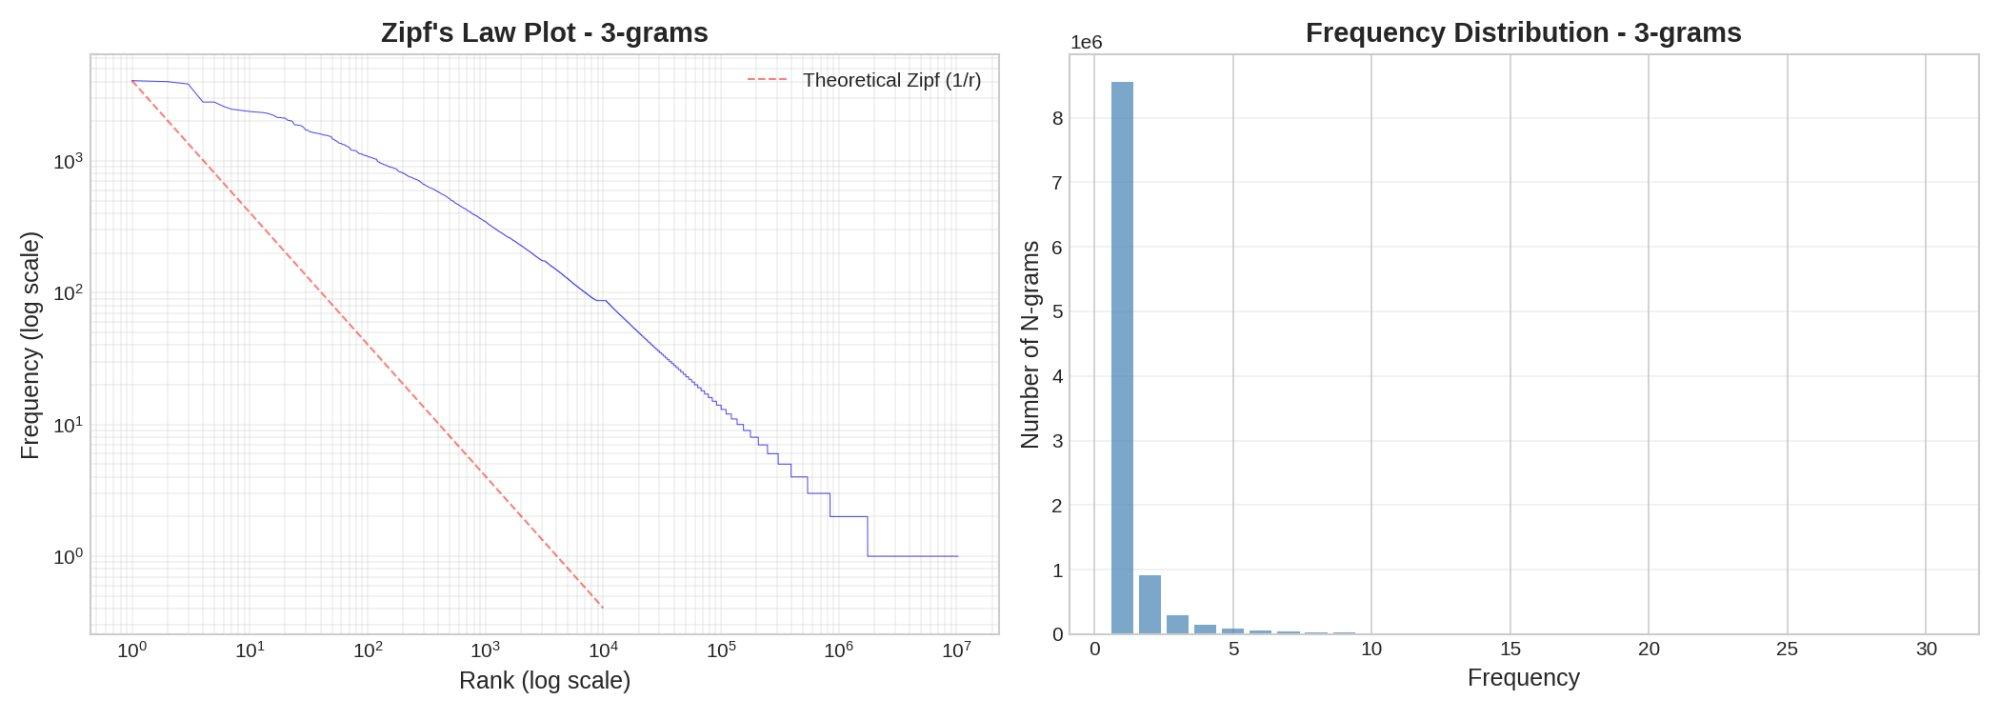
\includegraphics[width=0.9\linewidth]{figures/image8.jpg}
\caption{Trigram Zipf's Law Plot and Frequency Distribution}
\label{fig:trigram_zipf}
\end{figure}

Trigrams show steeper Zipf decay than bigrams, with the vast majority appearing only once. The frequency histogram is even more skewed, with over 8.5 million hapax legomena.

\textbf{Top Trigrams:} Figure~\ref{fig:trigram_top} shows the 20 most frequent trigrams.

\begin{figure}[H]
\centering
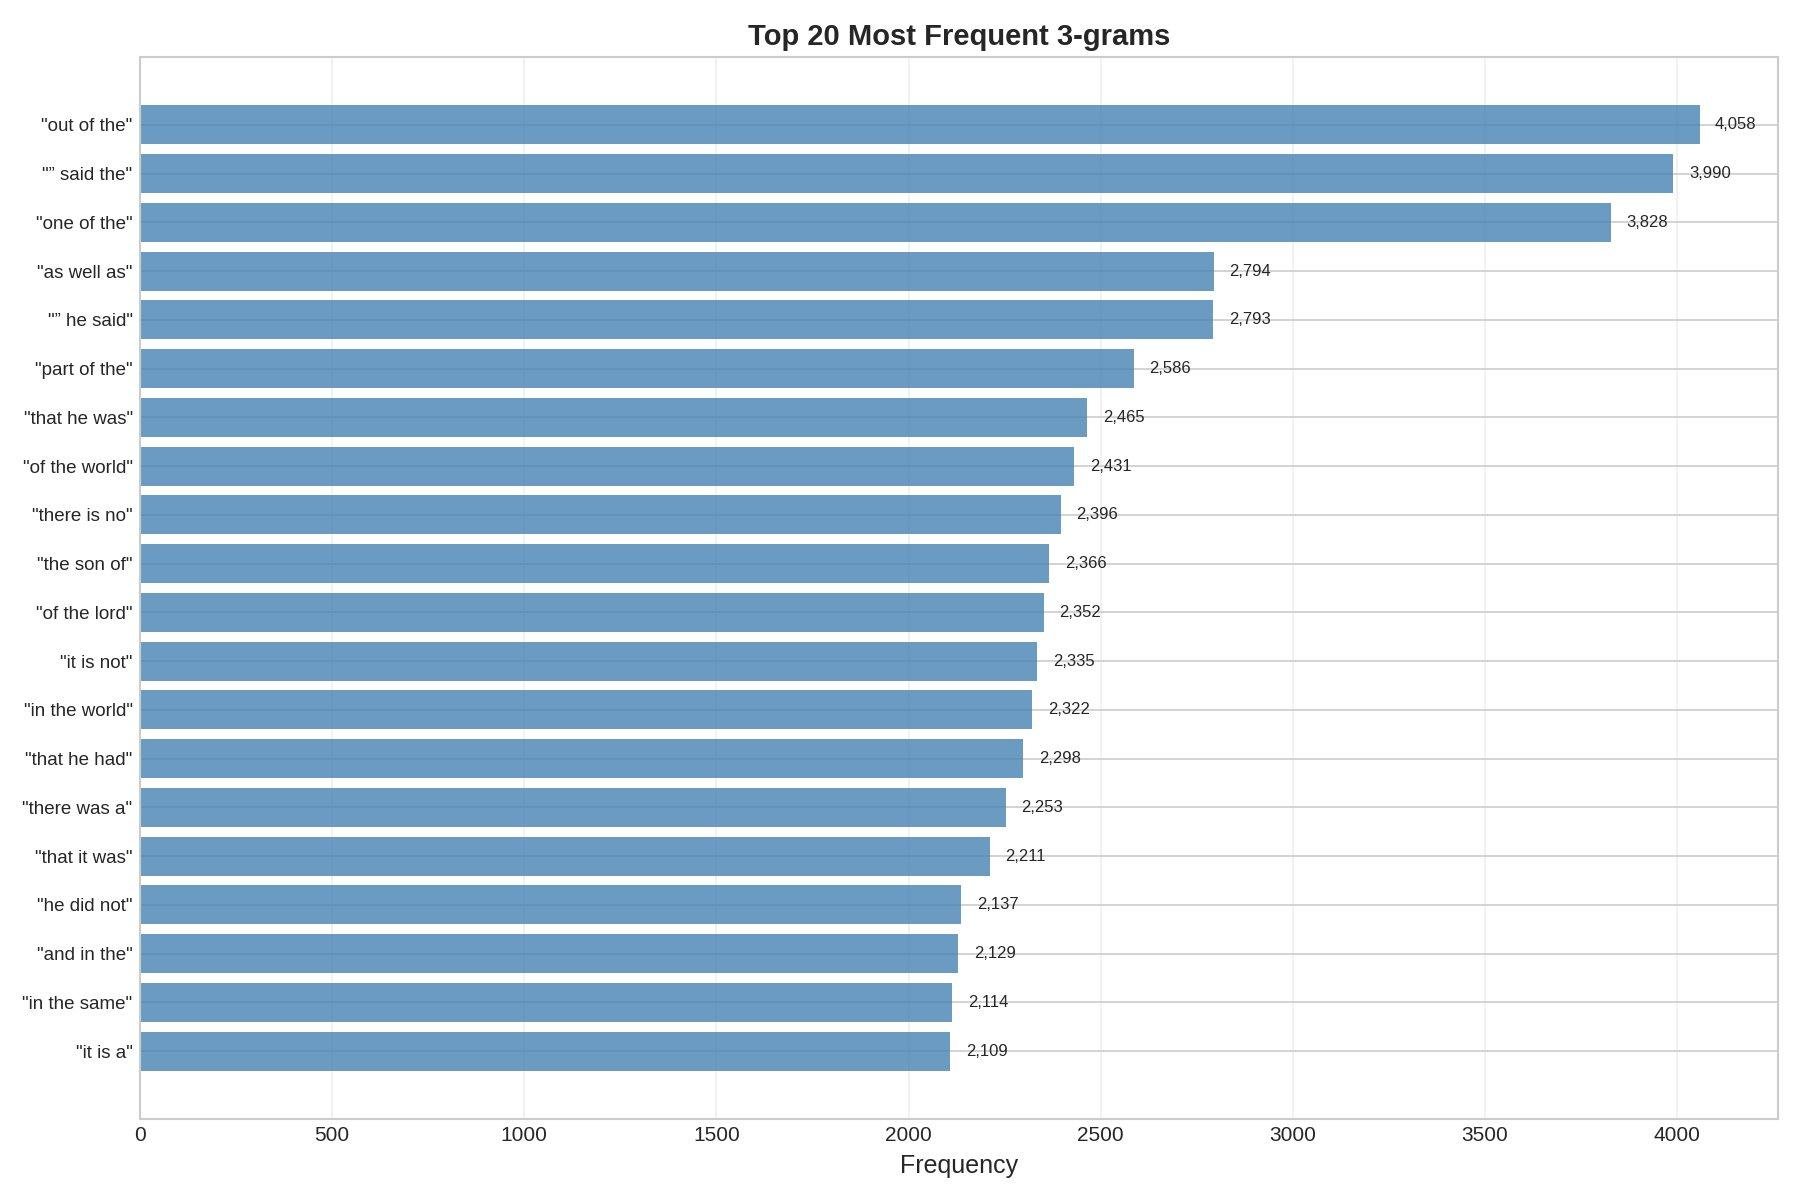
\includegraphics[width=0.9\linewidth]{figures/image3.jpg}
\caption{Top 20 Most Frequent Trigrams}
\label{fig:trigram_top}
\end{figure}

The most frequent trigram is ``out of the'' with 4,058 occurrences, followed by phrases like ``one of the'' (3,828) and ``as well as'' (2,794). Unlike bigrams, trigrams show more semantic content.

\textbf{Statistics Summary:} Figure~\ref{fig:trigram_stats} presents the trigram analysis summary.

\begin{figure}[H]
\centering
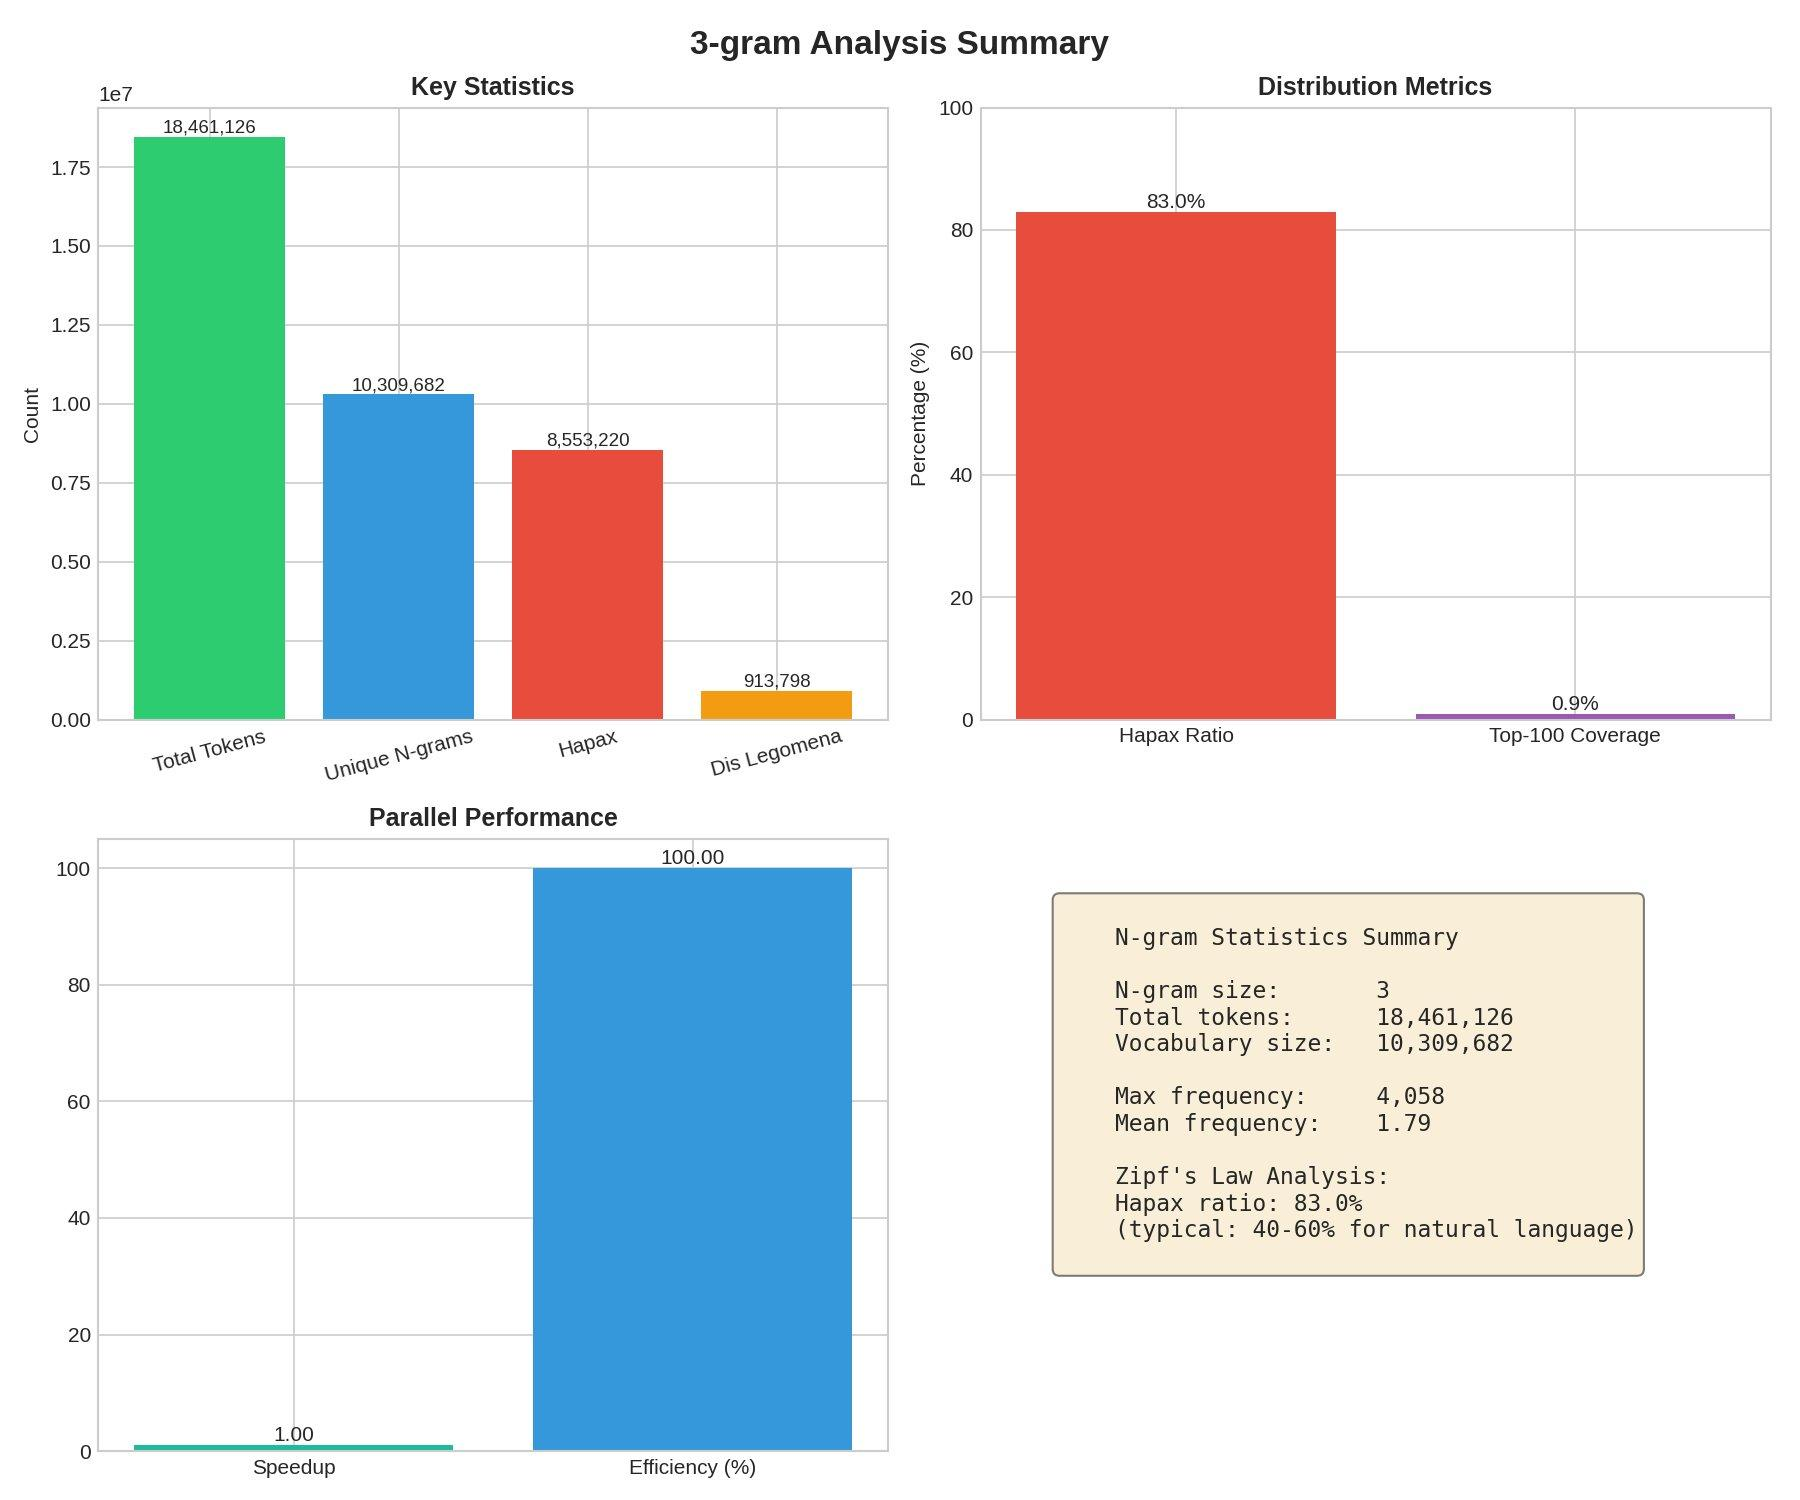
\includegraphics[width=0.9\linewidth]{figures/image7.jpg}
\caption{Trigram Analysis Summary}
\label{fig:trigram_stats}
\end{figure}

Key statistics: 18,461,126 total tokens, 10,309,682 unique trigrams (3x more than bigrams), 83.0\% hapax ratio (vs 67.9\% for bigrams), mean frequency only 1.79. The much larger vocabulary explains the reduced parallel efficiency.

\subsection{Bigram vs Trigram Comparison}

Comparing bigrams and trigrams reveals important differences:

\begin{itemize}
\item \textbf{Vocabulary size:} Trigrams have 3x more unique entries (10.3M vs 3.4M), requiring larger hash tables.
\item \textbf{Hapax ratio:} Trigrams have 83\% hapax vs 67.9\% for bigrams, indicating sparser distributions.
\item \textbf{Maximum frequency:} Bigram max is 139,216 vs only 4,058 for trigrams.
\item \textbf{Parallel efficiency:} Bigrams achieve 2.7-3.9x speedup vs 1.0-1.95x for trigrams.
\item \textbf{Best strategy:} Document Level wins for bigrams; Fine-grained-locking wins for trigrams.
\end{itemize}

The larger vocabulary and sparser distribution of trigrams creates more memory pressure and reduces cache efficiency, explaining the lower parallel speedup.

\section{Conclusions}

\subsection{Results Analysis}

The project demonstrated the effectiveness of OpenMP parallelization for n-gram counting, with performance varying significantly between bigrams and trigrams. For bigram analysis, the Document Level TLS strategy achieved the best results with speedups up to 3.9x at high workloads, showing good scalability across different thread counts. Trigram counting proved more challenging due to the larger vocabulary size, with Fine-grained-locking emerging as the best strategy despite reaching only 1.95x speedup. Both analyses confirmed that natural language text follows Zipf's Law, with trigrams exhibiting higher hapax ratios (83\%) compared to bigrams (68\%), indicating sparser frequency distributions as n-gram size increases.

\subsection{Performance Bottlenecks}

Analysis identified several factors limiting parallel scalability. Memory bandwidth represents the primary bottleneck, as hash table operations are inherently memory-bound and cannot fully exploit additional CPU cores. Cache efficiency degrades significantly for trigrams, where hash tables containing over 10 million entries far exceed L3 cache capacity, causing frequent main memory accesses. The TLS-based strategies suffer from merge overhead when combining large local histograms at the end of parallel execution. Additionally, vocabulary sparsity increases exponentially with n-gram size, creating more unique entries and reducing the benefit of parallel counting.

\subsection{Future Developments}

Several improvements could enhance performance in future iterations. SIMD vectorization could accelerate string comparison operations during n-gram construction. Concurrent hash maps would eliminate the merge phase entirely, removing a sequential bottleneck. Memory-mapped file I/O could improve loading performance for large corpora. GPU acceleration using CUDA would enable massive parallelism for vocabulary sizes that overwhelm CPU caches. Finally, approximate counting techniques such as Count-Min Sketch could trade perfect accuracy for dramatically reduced memory usage.

\subsection{Final Considerations}

The project confirms that parallelization benefits depend strongly on problem characteristics. Bigram counting achieves good speedups in the range of 3-4x, making it well-suited for parallel execution on multi-core systems. Trigram counting is more challenging due to vocabulary explosion, requiring careful strategy selection. The results suggest that TLS-based approaches work best for smaller vocabularies where merge overhead is manageable, while fine-grained locking scales better for larger vocabularies by distributing contention across multiple shards. The combination of OpenMP parallelization with efficient data structures makes n-gram counting practical for large-scale text analysis applications.

\begin{thebibliography}{9}

\bibitem{stanford_nlp}
Stanford NLP - N-gram Language Models.
\url{https://web.stanford.edu/~jurafsky/slp3/3.pdf}

\bibitem{openmp}
OpenMP Specifications.
\url{https://www.openmp.org/specifications/}

\bibitem{gutenberg}
Project Gutenberg.
\url{https://www.gutenberg.org/}

\bibitem{zipf}
Wikipedia - Zipf's Law.
\url{https://en.wikipedia.org/wiki/Zipf%27s_law}

\bibitem{repo}
Project Repository.
\url{https://github.com/MattiaManneschi/N-gram-Histograms}

\end{thebibliography}

\end{document}
